\section{Evaluation}
\label{sec:evaluation}

In this section, we analyze the performance of our algorithm
to check the equivalence of context-free session types. 
To do so, we have implemented the algorithm we have presented
thus far (sketched in Listings~\ref{lst:toGrammar}, 
\ref{lst:prune}, \ref{lst:algorithm}) 
in Haskell, and used Haskel compiler 
Glasgow Haskell Compiler, GHC version 8.6.3, from which we have 
obtained the running times we present throughout this section.
The machine used for the evaluation was a Mac mini at 3,6 GHz Intel 
Core i3 with 8 GB of memory. 

At this stage, we were aiming to analyze the performance of
our type equivalence checking algorithm, when we came across 
a particular test whose context-free session types where:
\begin{equation}
\label{ex:chaotic}
	\begin{aligned}
		S &\triangleq \mu x . \&\{ \mathsf{add}: x;x; !\,\intk,
							       \mathsf{const}: ?\,\intk;!\in\intk,
							       \mathsf{mult}: x;x;!\,\intk\}\\
		T &\triangleq \mu x . \&\{ \mathsf{add}: x;x,
							  	   \mathsf{const}: ?\,\intk,
							       \mathsf{mult}: x;x\}; !\,\intk
	\end{aligned}
\end{equation}
\lstinline{equivalent S T} took 4810.21 seconds to decide the equivalence
positively. This would not be a reasonable amount of time for a
feasible compiler. Hence, we started to pave the way to improve the
running times. For this purpose, we propose:
\begin{enumerate}
	\item to iterate the simplification stage until a fixed point
	on the \emph{simplest children nodes} is reached;
	\item to consider a double ended queue, where \emph{promising} 
	children nodes would be prepended, as opposed to enqueuing 
	all new nodes.
\end{enumerate}

If, in one hand, we believe that the computation of the expansion
tree can be speeded up by extending the simplification phase, on 
the other hand we believe that a double ended queue will allow us to 
prioritize nodes that potentially allow us to reach an empty node faster.
The latter is obtained by prepending nodes that are already empty or, 
either, whose pairs $(\vec X, \vec Y)$ are such that $|\vec X|\leq 1$
and $|\vec Y| \leq 1$.
For the former, we need to check that a fixed point exists and,
hence, for a given node $N$, we are able to compute the 
\emph{simplest} children nodes derived from $N$ using the
simplification rules.

\begin{theorem}
\label{thm:fixed_point}
	The simplification function that results from applying the reflexive,
	congruence, and \BPA\ rules, has a fixed point in the complete partial
	ordered set \lstinline{Set (Node,Ancestors)}, where the set of ancestors
	is supposed to be fixed and equal to $A$.
\end{theorem}

Throughout the proof of Theorem~\ref{thm:fixed_point}, we will abuse 
notation and denote the application of simplification rules
to nodes or to elements of $\text{\lstinline{Set (Node,Ancestors)}}$
in the same way, when no ambiguities arise.

\begin{proof}
	Consider the order 
	$\leqSets$ defined in $\text{\lstinline{Set (Node,Ancestors)}}
	\times \text{\lstinline{Set (Node,Ancestors)}}$ as follows:
	$S_1 \leqSets S_2$ if $|S_1| \leq |S_2|$ and
	exists an injective map $\sigma : S_1 \rightarrow S_2$ s.t.\  
	$\sigma(N_1,A) = (N_2,A)$ with $N_2\subseteq N_1$.\\
	
	\noindent\textbf{$\leqSets$ is a partial order:} The proof that
	$\leqSets$ is reflexive and transitive is straightforward. 
	To prove that it is 
	antisymmetric, assume that $S_1\leqSets S_2$ and $S_2 \leqSets S_1$.
	This means that $|S_1|=|S_2|$ and, furthermore, the maps 
	$\sigma_1 : S_1 \rightarrow S_2$ and $\sigma_2 : S_2 \rightarrow S_1$
	are bijective. Notice that $\sigma_1\circ \sigma_2$  
	is the identity map, otherwise we could consider $(N,A)\in S_2$
	where $N$ is minimal w.r.t.\ inclusion and s.t.\
	$(\sigma_1\circ \sigma_2)(N,A) \neq (N,A)$, i.e.,
	$(\sigma_1\circ \sigma_2)(N,A) = (N',A)$ with $N'\subseteq N$ 
	for some $(N',A)\in S_2$;
	due to the minimality of $N$, we would have 
	$(\sigma_1\circ \sigma_2)(N',A) = (N',A)$, which would contradict the
	injectivity of $\sigma_1\circ \sigma_2$. For the same reason 
	$\sigma_1\circ \sigma_2$ is also the identity map, and so, since
	$\sigma_i (N,A) = (N',A)$ is such that $N'\subseteq N$, we shall 
	have $\sigma_i (N,A) = (N,A)$. Hence, $S_1=S_2$.\\
	
	\noindent\textbf{The simplification function is order-preserving:}
	To prove that the reflexive rule preserves the order, let $S_1$ and 
	$S_2$ be s.t.\ $S_1\leqSets S_2$ and let us prove that 
	$\text{\lstinline{reflex}} S_1\leqSets\text{\lstinline{reflex}}S_2$.
	%Start noticing that $|S| = |\text{\lstinline{reflex}} S|$, hence
	%the number of children nodes is preserved by using the reflexive
	%rule, let us analyze each case. 
	Let $(N,A)\in \text{\lstinline{reflex}} S_1$
	and notice that there exists $(N_1,A)\in S_1$, such that
	$\text{\lstinline{reflex}} N_1 = N $, and so,
	in $S_2$ there is $(N_2,A)=\sigma(N_1,A)$ s.t. $N_2\subseteq N_1$. 
	Since $N_2\subseteq N_1$, we have
	$\text{\lstinline{reflex}} N_2 \subseteq
    \text{\lstinline{reflex}} N_1 = N$.
	
	The same reasoning applies to prove that if $S_1\leqSets S_2$ then 
	$\text{\lstinline{congruence} } S_1\leqSets\text{\lstinline{congruence} }S_2$.
	
	To prove that \lstinline{bpa1} also preserves the order, just start
	noting that 
	$S \subseteq \text{\lstinline{bpa1} }S$. Assume that 
	$S_1\leqSets S_2$, let $(N,A)\in \text{\lstinline{bpa1} }S_1$, 
	and denote by $(N_1,A)\in S_1$ and $(\vec X,\vec Y)\in N_1$  
	the node and the pair whose simplification 
	led to $(N,A)$. We know that there exists $(N_2,A)\in S_2$
	such that $N_2 \subseteq N_1$. If $(\vec X,\vec Y)\in N_2$,
	then the \lstinline{bpa1} simplification of $N_2$ with
	the pair $(\vec X,\vec Y)$ generates 
	$(N',A)\in \text{\lstinline{bpa1} }S_2$ such that 
	$N'\subseteq N$. On the other hand, if 
	$(\vec X,\vec Y)\not \in N_2$, then $N_2\subseteq N$ 
	and, since  $S_2 \subseteq \text{\lstinline{bpa1} }S_2$,
	$(N_2,A)\in \text{\lstinline{bpa1} }S_2$ is such that
	$N_2\subseteq N$.
	
	The same reasoning applies to \lstinline{bpa2}. Having proved
	that each simplification function preserves the order, and
	since the simplification procedure results from the successive 
	application of this rules, we have proved that the simplification
	function also preserves the order.\\
	
	\noindent\textbf{$(\text{\lstinline{Set (Node,Ancestors)}}, \leqSets)$
	is a lattice:} Given 
	$S_1, S_2\in \text{\lstinline{Set (Node,Ancestors)}}$:
	\begin{itemize}
		\item $S_1 \cup S_2$ is an upper bound;
		\item $S_1 \cap S_2$ is a lower bound.
	\end{itemize}
	
	\noindent\textbf{$(\text{\lstinline{Set (Node,Ancestors)}}, \leqSets)$
	is a complete lattice:} Given 
	$\mathcal{B}\subseteq \text{\lstinline{Set (Node,Ancestors)}}$:
	\begin{itemize}
		\item $\bigcup_{S\in \mathcal{B}} S$ is an upper bound;
		\item $\bigcap_{S\in \mathcal{B}} S$ is a lower bound.
	\end{itemize}
	
	Using the fixed point theorem from Tarski~\cite{tarski1955lattice}, 
	we conclude that the simplification function has a
	fixed point in $\text{\lstinline{Set (Node,Ancestors)}}$.
%	Consider the order 
%	$\leqSets$ defined in $\text{\lstinline{Set (Node,Ancestors)}}
%	\times \text{\lstinline{Set (Node,Ancestors)}}$ as follows:
%	$S_1 \leqSets S_2$ if $|S_1| \geq |S_2|$ and:
%	\begin{itemize}
%		\item if $|S_1|=|S_2|$ then exists a bijection 
%			$\sigma : S_1 \rightarrow S_2$ s.t.\  
%			$\sigma(N,A) = (N',A)$ with $N\subseteq N'$;
%		\item if $|S_1| > |S_2|$ then for each 
%			$(N,A)\in S_1$ exists $(N',A')\in S_2$ s.t.\ 
%			$(N,A) \preceq (N',A')$,
%	\end{itemize}
%	where $|S|$ represents the number of elements of $S$ and
%	$\leqNAS$ is defined on $\text{\lstinline{(Node,Ancestors)}}
%	\times \text{\lstinline{(Node,Ancestors)}}$ as follows:
%	$(N,A) \leqNAS (N',A')$ if $A=A'$ and for each 
%	$(\vec X,\vec Y)\in N$ either:
%	\begin{itemize}
%		\item $(\vec X, \vec Y)\in N'$, or
%		\item exists $(\vec{X'},\vec{Y'})\in N'\setminus N$ s.t.
%			  $\size(\vec X, \vec Y) < \size(\vec{X'},\vec{Y'})$,
%	\end{itemize}
%	where, finally, $\size (\vec X, \vec Y) = \mathsf{min}\{s(\vec X), s(\vec Y)\}$
%	and 
%	\[ s(\vec X Y) = 
%	\begin{cases}
%		|\vec X Y| & \text{if $Y$ is normed}\\
%		|\vec X| & \text{otherwise}
%	\end{cases}
%	\]
%	
%	\noindent\textbf{$\leqSets$ is a partial order:} The proof that
%	$\leqSets$ is reflexive and transitive is straightforward. 
%	To prove that it is 
%	antisymmetric, assume that $S_1\leqSets S_2$ and $S_2 \leqSets S_1$.
%	This means that $|S_1|=|S_2|$ and, so, let 
%	$\sigma_1 : S_1 \rightarrow S_2$ and $\sigma_2 : S_2 \rightarrow S_1$
%	be the corresponding bijections. Notice that $\sigma_1\circ \sigma_2$  
%	is the identity map, otherwise we could consider $(N,A)\in S_2$
%	where $N$ is minimal w.r.t.\ inclusion and s.t.\
%	$(\sigma_1\circ \sigma_2)(N,A) \neq (N,A)$, i.e.,
%	$(\sigma_1\circ \sigma_2)(N,A) = (N',A)$ with $N'\subseteq N$ 
%	for some $(N',A)\in S_2$;
%	due to the minimality of $N$, we would have 
%	$(\sigma_1\circ \sigma_2)(N',A) = (N',A)$, which would contradict the
%	injectivity of $\sigma_1\circ \sigma_2$. For the same reason 
%	$\sigma_1\circ \sigma_2$ is also the identity map, and so, since
%	$\sigma_i (N,A) = (N',A)$ is such that $N'\subseteq N$, we shall 
%	have $\sigma_i (N,A) = (N,A)$. Hence, $S_1=S_2$.	
\end{proof}

We have tested the several combination of the previous proposals
in our algorithm on a batch of 138 tests. The results are presented 
in Figure~\ref{fig:results}.

\begin{figure}[h]
	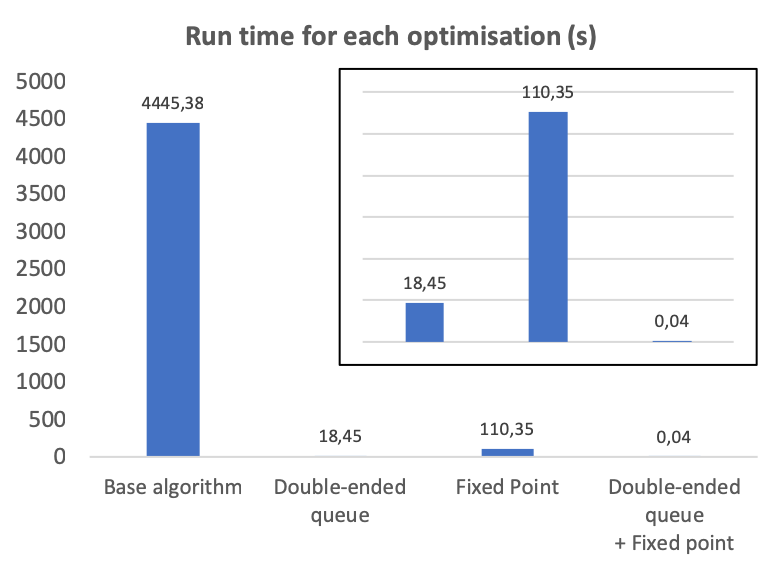
\includegraphics[height=4.8cm]{img/run_time}	\qquad 
	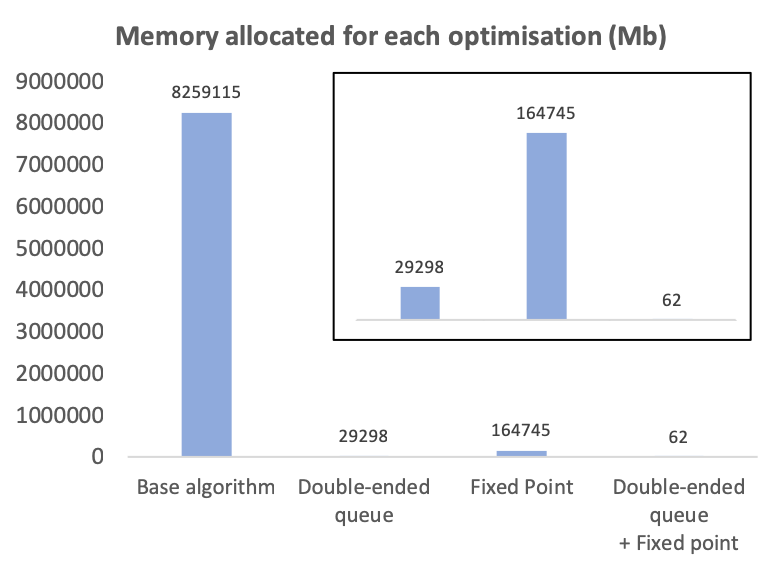
\includegraphics[height=4.8cm]{img/memory_alloc}	
	\caption{Test results: running times (on the left) and
	memory allocated (on the right) checking the equivalence 
	of context-free session types in 138 tests.}
	\label{fig:results}
\end{figure}

The running times and memory allocated presented in 
Figure~\ref{fig:results}, exhibit an improvement on more 
than 12000000\%. The decision for the equivalence of our particular
example in~\eqref{ex:chaotic} took now only 0.01
seconds. For this reasons, our proposal for an
algorithm to check the equivalence of context-free session types 
stands on adapting the simplification stage to enable double ended 
enqueueing and the computation of a fixed point at the
simplification phase. Listing~\ref{lst:enhanced} presents
an enhanced version of the simplification stage coping the new
proposals.
\begin{lstlisting}[caption={Haskell code for the adapted simplification
                   stage of the improved algorithm to check the 
                   equivalence of context-free session types},
                   label={lst:enhanced} ,captionpos=b] 
simplify :: Productions -> Ancestors ->  Node -> NodeQueue -> NodeQueue
simplify g a n q = foldr enqueueNode (Queue.dequeue q) m'
  where m' = findFixedPoint g (Set.singleton (n,a))

enqueueNode :: (Node,Ancestors) -> NodeQueue -> NodeQueue
enqueueNode (n,a) q
 | Set.null n           = Queue.priorityEnqueue (n,a) q
 | maximumLength n == 1 = Queue.priorityEnqueue (n,a) q
 | otherwise            = Queue.enqueue (n,a) q

findFixedPoint :: Productions -> Set.Set (Node,Ancestors) -> 
                  Set.Set (Node,Ancestors)
findFixedPoint g nas
  | nas == nas' = nas
  | otherwise = findFixedPoint g nas'
  where nas' = if allNormed p
                then foldr (apply p) nas [reflex,congruence,bpa2]
                else foldr (apply p) nas [reflex,congruence,bpa1,bpa2]
\end{lstlisting}



%%% Local Variables:
%%% mode: latex
%%% TeX-master: "main"
%%% End:
